\section{Machine Learning Fundamentals}
%%%%%%%%%%%%%%%%%%%%%%%%%%%%%%%%%%%%%%%%%%%%%%%%%%%%%%%%%%%%%%%%%%%%%%%%%%%%%%%%
This section aims at providing a non-exhaustive coverage of the basics of
\gls{ML} which can be applied to all \gls{ML} algorithms. This section starts by
defining what is meant when it is said that an algorithm ``learns". The types of
datasets that may be encountered in the application of these learning algorithms
are then briefly covered to provide insight into the potential applications
which are not covered in this review. This is then followed by making the
distinction between the goal of fitting training data and the goal of finding
patterns that generalize to new data. Finally, a very common concept in machine
learning is covered: \textit{hyperparameters}, which are \textit{settings} of a
learning algorithm which must be determined outside the learning algorithm
itself.

\subsection{Learning algorithms\label{ssec:learning_algo}}
%%%%%%%%%%%%%%%%%%%%%%%%%%%%%%%%%%%%%%%%%%%%%%%%%%%%%%%%%%%%%%%%%%%%%%%%%%%%%%%%
Generally speaking, a machine learning algorithm is a procedure for learning
from data. However correct this definition is, it provides little insight into
the relevant concepts in the field. A more succint definition is provided by
Mitchell~\cite{Mitchell97LearningAlgorithm}:

\begin{fancyquotes}
    A computer program is said to learn from experience $E$ with respect
    to some class of tasks $T$ and a performance measure $P$, if its performance
    at tasks in $T$, as measured by $P$, improves with experience $E$.
\end{fancyquotes}

This definition introduces the general entities which are present during all
machine learning tasks. The entities will not be formally defined in the
following sections as it is far outside the scope of this literature, and is
philosophical in nature. This section will instead cover examples of each which
will provide practical insight on which the reader can build their knowledge.

\subsubsection{The Task, $T$}
%%%%%%%%%%%%%%%%%%%%%%%%%%%%%%%%%%%%%%%%%%%%%%%%%%%%%%%%%%%%%%%%%%%%%%%%%%%%%%%%
There exists a plethora of tasks which humanity has applied learning algorithms
to during the timeline of the field. It is common for \gls{ML} practitioners to
originate from domains outside that of computer science, in order to assess the
feasibility of existing algorithms in their domain. There is however a question
that often presents itself to specialists in their respective fields when they
consider applying \gls{ML} to the existing problems in their field. Why should a
specialist opt for solving problems with \gls{ML} that have been solved using
tried and true techniques in their domain of expertise? Goodfellow et al.
\cite{Goodfellow-et-al-2016} provides an insightful response to this:

\begin{fancyquotes}
    Machine learning enables us to tackle tasks that are too difficult
    to solve with fixed programs written and designed by human beings. From a
    scientific and philosophical point of view, machine learning is interesting
    because developing our understanding of it entails developing our
    understanding of the principles that underlie intelligence.
\end{fancyquotes}

An example of a field which has undergone dramatic changes in a short period of
time, with the advent of \gls{DL} and modern hardware, is \gls{CV}. Mahony et
al. discuss this in their paper with a focus on comparing \gls{DL} and \gls{CV}
\cite{Mahony-et-al-2020}. Their paper concludes that many \gls{CV} techniques
invented in the 20 years preceding the paper have become irrelevant as a result
of \gls{DL}. However, they emphasise on the importance of the knowledge
established in those 20 years, arguing that \textit{``knowledge is never
obsolete"}, as it provides specialists with more tools and intuition when
addressing problems. Some typical applications of \gls{CV} are detailed and
although these may be outperformed by \gls{DL}, relying on \gls{DL} in some
cases is overkill. They also point out some hybrid approaches between \gls{DL}
and \gls{CV} which synergize, saying that \gls{CV} provides improved performance
in \gls{DL} by reducing training time. This emphasises that specialists should
not expect an end-all solution from \gls{ML} in addressing their domain-specific
problems, but rather as mentioned by Goodfellow et al., strive for a better
understanding of the principles that underlie intelligence, and by extension,
those that underlie the practitioners domain-specific problems.

\begin{itemize}
    \item \textbf{Classification}: In this task, the learning algorithm is
    expected to produce a function $f: \mathbb{R^n}\rightarrow
    \{1,...,k\}$. When $y=f(\mathbf{x})$, the model assigns a provided
    input, $\mathbf{x}$ to a category identified by numeric code $y$. An
    example of this would be the mapping of a grayscale image,
    $\mathbf{x}\in\mathbb{R}^2$ to a value corresponding to a numerical
    encoding $f:\mathbb{R}^n\rightarrow\{\textrm{Cat},\;\textrm{Dog}\}$.
    \item \textbf{Classification with missing inputs}: Classification becomes
    more challenging when the input measurements to the model are not
    guaranteed to always be the same. In this situation the algorithm must
    learn the set of all function mappings arising from the possible
    combinations of input vectors that arise from missing subsets of
    inputs in $\mathbf{x}$. An example of this would be the classification
    of a diagnosis in medicine, as depending on the invasiveness of
    certain procedures, different subsets of measurements are available.
    \item \textbf{Regression}: In this task, the learning algorithm is expected
    to predict a continuous numerical value for a given input. This is
    done by learning a function $f: \mathbb{R}^n\rightarrow\mathbb{R}$.
    the formulation is similar to that of classification, except for the
    output format. An example of this would be learning of a function to
    predict the expected returns for a given investment given the state of
    the market, as is common is algorithmic trading.
    \item \textbf{Transcription}: This type of task involves the learning
    algorithm observing a relatively unstructured input and transcribing
    it into some discrete textual form. An example of this is the
    transcription of an audio waveform containing speech into text.
    \item \textbf{Machine translation}: In machine translation, the already
    structured input is mapped into a different language. This is common
    in the field of \gls{NLP}, where languages are translated between, for
    example English and French. This however is not limited to natural
    languages but can also be applied to programming languages for
    example.
    \item \textbf{Structured output}: This task entails those where the output
    is a vector or a data structure which details important relationships
    between the contained elements. This task subsumes the prior two of
    transcription and machine translation. An example of this would be the
    parsing of grammatical structure of a natural language sentence,
    addressed in \gls{NLP} and demonstrated by Collobert
    \cite{pmlr-v15-collobert11a}.
    \item \textbf{Anomaly detection}: In this task, a learning algorithm learns
    to sift through a set of events and classify events that are anomalous
    in nature. These algorithms have been applied to credit card companies
    in detection of fraud \cite{DBLP:journals/corr/abs-2108-10005}, and in
    safety in the aviation industry \cite{Janakiraman2016, Basora2019}.
    \item \textbf{Synthesis and sampling}: In this task, learning algorithms
    generate \textbf{new} examples which appear to be drawn from the same
    underlying distribution as, but are not present in the training data.
    A recent example around which a lot of research is being done is the
    \gls{GPT-3} which is able to produce human-like text, given prompts as
    input \cite{DBLP:journals/corr/abs-2005-14165}.
    \item \textbf{Imputation of missing values}: In this task, the learning
    algorithm is given some input $x\in\mathbb{R}$ with some elements
    $x_i$ missing. The algorithm must then make predictions for the
    missing values. Emmanuel et al. discuss the latest methods in
    \gls{ML} that address this task~\cite{Emmanuel2021}. A recent example of
    imputation of missing frames for the purpose of adding frames to videos
    is \gls{RIFE} \cite{huang2020rife}.
    \item \textbf{Denoising}: In this learning task, the machine learning
    algorithm learns to generate a clean example $\mathbf{x}\in\mathbb{R}^n$
    from a corrupted sample $\tilde{\mathbf{x}}\in\mathbb{R}^n$. Generally
    speaking the learner is predicting the probability distribution
    $p(\mathbf{x}|\tilde{\mathbf{x}})$.
    \item \textbf{Density estimation} or \textbf{probability mass function estimation}
    involves the task of learning a function $p_\text{model}:\mathbb{R}^n\rightarrow{}\mathbb{R}$,
    where $p_\text{model}(\mathbf{x})$ is interpreted as a probability distribution function
    from which $\mathbf{x}$ was drawn. Effectively the algorithm learns the
    structure of the data that it has been provided with. Most of the
    aforementioned tasks involve learning this distribution function, at least
    implicitly. For example for the missing value imputation task, if $x_i$ is
    missing, and all other values $x_{-i}$ are given, then the algorithm learns
    the distribution $p(x_i|\mathbf{x}_{-i})$ which involves $p(\mathbf{x})$
    implicitly.
\end{itemize}
%An ongoing trend in society is the augmentation of responsibility in intelligent
%algorithms through autonomy, evident by the advent of semi-autonomous cars,
%autonomous cyber-security \cite{Taeihagh2019}, autonomous industrial site
%inspection\footnote{\url{https://newsroom.ibm.com/Boston-Dynamics-and-IBM-Join-Forces-to-Bring-Mobile-Edge-Analytics-to-Industrial-Operations}},
%and autonomous supply-chain
%management\footnote{\url{https://www.forbes.com/sites/stevebanker/2021/04/01/amazon-supply-chain-innovation-continues/}},
%to name a few.

%This section reviews the current ongoing research in the field of machine
%learning as a whole. First the main categories:

\subsubsection{The Performance, $P$\label{sec:ML-performance}}
%%%%%%%%%%%%%%%%%%%%%%%%%%%%%%%%%%%%%%%%%%%%%%%%%%%%%%%%%%%%%%%%%%%%%%%%%%%%%%%%
In order to assess the performance of our learning algorithm in task $T$,
we must have some quantitative measure of performance $P$ with which we steer
the algorithm towards the desired behaviour. $T$ and $P$ in this way are
coupled, and must $P$ must be chosen according to $T$. In this way it can be
unclear to the \gls{ML} practitioner what $P$ should be chosen.

Firstly, it is worth considering the true goal of the learning algorithm. We
wish for it to train according to some dataset such that it can generalize to
inputs that it has never seen before. After all, there is little worth in a
classification algorithm recognizing cats and dogs with 90\% accuracy on its
training dataset, if it performs with 20\% accuracy on an unseen \textbf{test}
dataset. This previously mentioned scenario is known as \textit{overfitting} and
is discussed in its own section later in the chapter. For this reason, the first
requirement on managing our dataset is presented, there must be some
\textbf{train-test split}. This is further complicated by the
\textbf{validation} dataset which is discussed later in the chapter.

Given that the input-output pair is $\{\gls{x_in_i}, \gls{y_true_i}\}$,
\gls{y_true_i} is commonly referred to as the \textit{ground truth}, and
$\hat{\mathbf{f}}(\gls{x_in_i})=\gls{y_pred_i}$ are referred to as the
\textit{predictor} and \textit{predicted output} respectively. The performance
in the form of a loss function \gls{J} (also referred to as an objective or cost
function in literature) is then a function of \gls{y_true_i} and
\gls{y_pred_i}, therefore $\gls{J}(\gls{y_pred_i}, \gls{y_true_i})$.

\gls{ML} often borrows from \textit{approximation theory} vector norm notation
($\ell(\cdot)_p=||\cdot||_p$) to simplify notation in performance metrics. See
\autoref{appendix:vector_norms} for the expressions of vector norms.

\textbf{Regression loss functions}
\begin{itemize}
    \item \textbf{\Gls{MSE}} is the average of the squared differences between
    predictions and the ground truth. It is only concerned with the average
    magnitude of errors irrespective of their direction. Due to the squaring,
    predictions which have greater errors are more heavily penalized. A
    beneficial mathematical property of \gls{MSE} is that gradients can be
    easily calculated.
    \begin{equation}
        \gls{J}_\text{\gls{MSE}} = \frac{1}{\gls{m}}\sum_{i=0}^{\gls{m}}||\gls{y_pred_i}-\gls{y_true_i}||^2_2
        \label{eq:MSE}
    \end{equation}
    \begin{equation*}
        \begin{aligned}
            \textrm{where, }
            \eqdesc{J}\text{,} \\
            \eqdesc{m}\text{,} \\
            \eqdesc{y_pred_i}\text{,} \\
            \eqdesc{y_true_i}\text{.} \\
        \end{aligned}
    \end{equation*}
    \item \textbf{L2 error} is the average of the differences between
    predictions and the ground truth. It is the same as \gls{MSE} but without
    the squaring. Like \gls{MSE}, the gradient can be easily calculated.
    \begin{equation}
        \gls{J}_\text{L2E} = \frac{1}{\gls{m}}\sum_{i=0}^{\gls{m}}||\gls{y_pred_i}-\gls{y_true_i}||_2
    \end{equation}
    \item \textbf{\Gls{MAE}} or \textbf{L1 loss} is the average of the sum of
    absolute differences between predictions and the ground truth. This measure
    is similar to \gls{MSE} in that it considers the magnitude of the errors and
    ignores their direction. However, \gls{MAE} is more difficult to compute
    gradients for, requiring linear programming. \gls{MAE} is also more
    resilient to large error values as a result of outliers, as it does not make
    use of a square.
    \begin{equation}
        \gls{J}_\text{MAE} = \frac{1}{\gls{m}}\sum_{i=0}^{\gls{m}}||\gls{y_pred_i}-\gls{y_true_i}||_1
        \label{eq:MAE}
    \end{equation}
    \item \textbf{\Gls{MBE}} is the sum of all differences between predictions
    and the ground truth. \gls{MBE} is not often used as a measure of the model
    error as high individual errors can produce a low \gls{MBE}. This metric is
    primarily used to measure the average bias of a prediction.
    \begin{equation}
        \gls{J}_\text{MBE} = \frac{1}{\gls{m}}\sum_{i=0}^{\gls{m}}\sum_{j=0}^{\gls{n_y}}(\gls{y_pred_ij}-\gls{y_true_ij})
    \end{equation}
    \begin{equation*}
        \begin{aligned}
            \textrm{where, }
            \eqdesc{n_y}\text{,} \\
            \eqdesc{y_pred_ij}\text{,} \\
            \eqdesc{y_true_ij}\text{.} \\
        \end{aligned}
    \end{equation*}
    \item \textbf{\Gls{MSLE}} can be interpreted as a measure of the ratio
    between predictions and the ground truth. This metric is used when it is
    desirable to achieve some relative measure of accuracy as opposed to an
    absolute. In other words, large and small discrepancies between the
    predicted and ground truth are dealt in a relative manner, resulting in
    similar loss value magnitudes.
    \begin{equation}
        \begin{aligned}
            \gls{J}_\text{MSLE} &= \frac{1}{\gls{m}}\sum_{i=0}^{\gls{m}}\sum_{j=1}^{\gls{n_y}}(\log{(\gls{y_true_ij}+1)} - \log{(\gls{y_pred_ij}+1)})^2 \\
            &= \frac{1}{\gls{m}}\sum_{i=0}^{\gls{m}}\sum_{j=0}^{\gls{n_y}}2\log(\frac{\gls{y_true_ij}+1}{\gls{y_pred_ij}+1})
        \end{aligned}
    \end{equation}
    \item \textbf{\Gls{CP}} or \textbf{\gls{CS}} is a measure of similarity
    between two non-zero vectors of an inner product space. The metric is
    defined as the cosine of the angle between the two vectors. The metric is
    bounded in the interval $[-1,1]$, -1 for opposing orientation and 1 for the
    same orientation. This is not often useful in some \gls{ML} tasks, so an
    alternative form known as the \textbf{\gls{CD}} is used instead. The
    relation between the metrics is $\text{\gls{CD}}=1-\text{\gls{CP}}$,
    bounding the error in the interval $[0,2]$.
    \begin{equation}
        \gls{J}_\text{\gls{CD}} =
        \frac{1}{\gls{m}}\sum_{i=0}^{\gls{m}}\bigg(1-\frac{\gls{y_true_i}\cdot{}\gls{y_pred_i}}{||\gls{y_true_i}||_2\cdot{}||\gls{y_pred_i}||_2}\bigg)
    \end{equation}
\end{itemize}

\textbf{Binary classification loss functions}
\begin{itemize}
    \item \textbf{Binary cross-entropy} i
    \begin{equation}
        L=-\sum_{i=1}^N\bigg(y_i\log(\hat{\mathbf{y}}_i)+(1-y_i)\log(1-\hat{\mathbf{y}}_i)\bigg)\label{eq:equation}
    \end{equation}
    \item Hinge loss
    \begin{equation}

    \end{equation}
    \item Squared hinge loss
\end{itemize}

\textbf{Multi-class classification loss functions}
\begin{itemize}
    \item Multi-class cross-entropy
    \begin{equation}
        L_{CE}=-\sum_{i=1}^N\sum_{j=1}^{M}y_{ij}\log(\hat{f}_j(\mathbf{x}_i))
    \end{equation}
    \item Hinge loss
    \item Squared hinge loss
\end{itemize}


\begin{itemize}
\end{itemize}

%With the
%In the case of classification, most metrics are derived from the confusion
%matric

\subsubsection{The Experience, $E$\label{sec:ML-experience}}
%%%%%%%%%%%%%%%%%%%%%%%%%%%%%%%%%%%%%%%%%%%%%%%%%%%%%%%%%%%%%%%%%%%%%%%%%%%%%%%%
Tasks provided to machine learning algorithms have different formulations based
on the experience made available. Learning algorithms can be broadly categorized
by the kind of experience that the algorithm has assess to during learning, from
which it is generally expected to learn some pattern of interest.

\begin{itemize}
    \item \textbf{Supervised learning} algorithms experience a dataset
    containing features (input) and labels (expected output), and are expected
    to learn a function mapping between the two. These algorithms can be further
    divided into two categories. \textbf{Classification algorithms} learn a
    mapping from an input to a discrete class label output. \textbf{Regression
    algorithms} learn a mapping from an input to a continuous value output.

%    example input-output pairs, otherwise referred to as the labelled training
%    data consisting of a set of training examples. The trained \textit{model} is
%    then provided an unseen $x$ for which it must estimate $y$ based on its
%    experience. Supervised models are further grouped into two subcategories,
%    classification and regression. \textbf{Classification} is the task of
%    mapping $x$ to a discrete output variable $y$ which determines the predicted
%    class based on the $x$. A simple example of this would be a $y$ in
%    $\mathbb{R}^2$ which determines whether the input image was a \textit{cat}
%    or a \textit{dog}. \textbf{Regression} is task of mapping $x$ onto a
%    continuous output variable $y$ which determines the value of some variable
%    of interest. An example of this would be the task of learning an
%    approximator to the function: $f(x)=x^2$.
    % Dimensionality reduction \cite{vogelstein2021supervised}

    \item \textbf{Unsupervised learning} algorithms experience a dataset
    containing only features and learn some useful properties of the structure
    of the dataset. This form of learning often addresses recognition problems
    in \textit{association} \& \textit{clustering} \cite{barlow1999ul}.

    \item \textbf{Semi-supervised} is a middle ground between supervised
    learning (in which all training data is labelled) and unsupervised learning
    (in which no label data is provided)~\cite{books/mit/06/CSZ2006}. Some
    example applications of this paradigm are dimensionality reduction
    ~\cite{Zhang2007}, clustering \cite{Bair2013}, and anomaly detection
    \cite{DBLP:journals/corr/abs-1805-06725}.

    \item \textbf{Reinforcement learning} are learning algorithms which rely
    exclusively on a series of reinforcements from its environment. These
    reinforcements can be positive (rewards) or negative (punishments). This
    category is discussed further in \autoref{ssec:RL}.
\end{itemize}

\subsection{Capacity, Overfitting and Underfitting}
%%%%%%%%%%%%%%%%%%%%%%%%%%%%%%%%%%%%%%%%%%%%%%%%%%%%%%%%%%%%%%%%%%%%%%%%%%%%%%%%
The primary objective in \gls{ML} is to find a model which performs well on
previously \textit{unseen data}, which has not been used during the training or
fitting of a model. This ability of the learning algorithm is referred to as its
ability to \textit{generalise}.

Typically the learning algorithm is trained according to a set of
\textit{training data} with which we aim at reducing the learners
\textbf{training error}. Due to this data having been directly used to optimise
the model during training, we cannot expect this error to be representative of
the model's \textbf{generalisation error}. In order to derive an estimate of the
generalisation error, we separate part of the initial data set into training and
\textbf{test data}, from which the \textbf{test error} is derived. Given some
assumptions about the \textbf{data-generating process}, such as the data being
\textbf{\gls{iid}}, it can be said that the training error is equal to the
expectation of the test error.

An important concept in \gls{ML} is the \textit{capacity} of the model. This is
defined informally as \textit{``a model’s [...] ability to fit a wide
variety of functions"}~\cite[p.~111-112]{Goodfellow-et-al-2016}. Machine learning
algorithms will generally perform their best when their capacity is appropriate
for the true complexity of the task they are expected to perform given the
available training data. Models with insufficient capacity will fail to perform
complex tasks and those with excessive capacity will perform complex tasks, but
they may overfit the training data.

One technique of controlling the capacity of an algorithm is to control its
\textbf{hypothesis space}, the set of possible functions that the algorithm may
use to solve the task at hand. In the case of a polynomial, such as the
arbitrary one seen in \autoref{fig:capacity-plots}, this effect can be
intuitively related to the models propensity to underfit and overfit a set of
training data.

\begin{figure}[htp]
    \centering
    % MIT License
%
% Copyright (c) 2021 Geoffrey H. Garrett
%
% Permission is hereby granted, free of charge, to any person obtaining a copy
% of this software and associated documentation files (the "Software"), to deal
% in the Software without restriction, including without limitation the rights
% to use, copy, modify, merge, publish, distribute, sublicense, and/or sell
% copies of the Software, and to permit persons to whom the Software is
% furnished to do so, subject to the following conditions:
%
% The above copyright notice and this permission notice shall be included in all
% copies or substantial portions of the Software.
%
% THE SOFTWARE IS PROVIDED "AS IS", WITHOUT WARRANTY OF ANY KIND, EXPRESS OR
% IMPLIED, INCLUDING BUT NOT LIMITED TO THE WARRANTIES OF MERCHANTABILITY,
% FITNESS FOR A PARTICULAR PURPOSE AND NONINFRINGEMENT. IN NO EVENT SHALL THE
% AUTHORS OR COPYRIGHT HOLDERS BE LIABLE FOR ANY CLAIM, DAMAGES OR OTHER
% LIABILITY, WHETHER IN AN ACTION OF CONTRACT, TORT OR OTHERWISE, ARISING FROM,
% OUT OF OR IN CONNECTION WITH THE SOFTWARE OR THE USE OR OTHER DEALINGS IN THE
% SOFTWARE.

%%%%%%%%%%%%%%%%%%%%%%%%%%%%%%%%%%%%%%%%%%%%%%%%%%%%%%%%%%%%%%%%%%%%%%%%%%%%%%%
% ACKNOWLEDGEMENTS
%%%%%%%%%%%%%%%%%%%%%%%%%%%%%%%%%%%%%%%%%%%%%%%%%%%%%%%%%%%%%%%%%%%%%%%%%%%%%%%
% Design and implementation of this diagram was inspired and adapted from:
% https://tex.stackexchange.com/questions/573127/tikz-plots-are-not-centered

%%%%%%%%%%%%%%%%%%%%%%%%%%%%%%%%%%%%%%%%%%%%%%%%%%%%%%%%%%%%%%%%%%%%%%%%%%%%%%%
% DEPENDENCIES
%%%%%%%%%%%%%%%%%%%%%%%%%%%%%%%%%%%%%%%%%%%%%%%%%%%%%%%%%%%%%%%%%%%%%%%%%%%%%%%
%\usepackage{tikz}
% \usetikzlibrary{positioning, decorations.text, calc}

%%%%%%%%%%%%%%%%%%%%%%%%%%%%%%%%%%%%%%%%%%%%%%%%%%%%%%%%%%%%%%%%%%%%%%%%%%%%%%%
% USER STYLING
%%%%%%%%%%%%%%%%%%%%%%%%%%%%%%%%%%%%%%%%%%%%%%%%%%%%%%%%%%%%%%%%%%%%%%%%%%%%%%%


%

%\tikzset{declare function={f(\x)=(-0.06*(\x-2)+0.5)*(\x-2)*(\x-2);}}% applied math style
%\foreach \Z in {1,...,42} {\pgfmathsetmacro{\X}{\Z/10}%
%\pgfmathsetmacro{\Y}{f(\X)+0.9*rnd}%
%\ifnum\Z=1
%\xdef\LstOne{(\X,\Y)}%
%\xdef\LstTwo{"(\X,\Y)"}%
%\else
%\xdef\LstOne{\LstOne (\X,\Y)}%
%\xdef\LstTwo{\LstTwo,"(\X,\Y)"}%
%\fi}%

\newcommand{\plotobservations} {
    \addplot[only marks, draw=blue, fill=blue] coordinates {
        (0.0, 2.5991314214589614)
        (0.4444444444444444, 1.3463852235976501)
        (0.8888888888888888, 1.3558966978583558)
        (1.3333333333333333, 0.1719351250071693)
        (1.7777777777777777, 0.0549444514647925)
        (2.2222222222222223, 0.45130282341732175)
        (2.6666666666666665, -0.04104830486674099)
        (3.1111111111111107, 0.3752375262271346)
        (3.5555555555555554, 1.034685792786699)
        (4.0, 1.430935111399573)
    };
}

\newcommand{\plottruedistribution}{
    \addplot[domain=-0.5:4.5, dashed, thin, gray!75] {
        (-0.06 * (x - 2) + 0.5) * (x - 2) * (x - 2)
    };


}

%%%%%%%%%%%%%%%%%%%%%%%%%%%%%%%%%%%%%%%%%%%%%%%%%%%%%%%%%%%%%%%%%%%%%%%%%%%%%%%%
\begin{subfigure}[b]{0.32\textwidth}
    \centering
    \begin{tikzpicture}
        \begin{axis}[
            xmin=-0.5,
            xmax=4.5,
            ymin=-0.5,
            ymax=3.5,
            ticks=none,
            xticklabels={\empty},
            yticklabels={\empty},
            ymajorgrids=false,
            xmajorgrids=false,
            axis line style = semithick,
            width=1.2\columnwidth]
            \plotobservations
            \plottruedistribution
            \addplot[domain=-0.5:4.5, thick, green!50!black] {
                1.3645283299815407 - 0.24329387 * x
            };
        \end{axis}
    \end{tikzpicture}
    \subcaption{Underfitting}
    \label{fig:underfitting}
\end{subfigure}\hfil
%%%%%%%%%%%%%%%%%%%%%%%%%%%%%%%%%%%%%%%%%%%%%%%%%%%%%%%%%%%%%%%%%%%%%%%%%%%
\begin{subfigure}[b]{0.32\textwidth}
    \centering
    \begin{tikzpicture}
        \begin{axis}[
            xmin=-0.5,
            xmax=4.5,
            ymin=-0.5,
            ymax=3.5,
            ticks=none,
            xticklabels={\empty},
            yticklabels={\empty},
            ymajorgrids=false,
            xmajorgrids=false,
            axis line style = semithick,
            width=1.2\columnwidth]
            \plotobservations
            \plottruedistribution
            \addplot[domain=-0.5:4.5, thick, green!50!black] {
                + 2.5332784046893866
                - 2.31697944 * x
                + 0.58870681 * x ^ 2
                - 0.01887639 * x ^ 3
            };
        \end{axis}
    \end{tikzpicture}
    \subcaption{Appropriate capacity}
    \label{fig:appropriate-capacity}
\end{subfigure}\hfil
%%%%%%%%%%%%%%%%%%%%%%%%%%%%%%%%%%%%%%%%%%%%%%%%%%%%%%%%%%%%%%%%%%%%%%%%%%%%%%%%%%%
\begin{subfigure}[b]{0.32\textwidth}
    \centering
    \begin{tikzpicture}
        \begin{axis}[
            xmin=-0.5,
            xmax=4.5,
            ymin=-0.5,
            ymax=3.5,
            ticks=none,
            xticklabels={\empty},
            yticklabels={\empty},
            ymajorgrids=false,
            xmajorgrids=false,
            samples=200,
            axis line style = semithick,
            width=1.2\columnwidth]
            \plotobservations
            \plottruedistribution
            \addplot[domain=-0.5:4.5, thick, green!50!black] {
                +2.599131312448361
                -10.588139742958015 * x^1
                +25.074367329152583 * x^2
                -12.832852119149837 * x^3
                -15.29078616509039 * x^4
                +10.350960340047243 * x^5
                +10.94777207200677 * x^6
                -14.543216443491573 * x^7
                +6.786937457668481 * x^8
                -1.5968672908165933 * x^9
                +0.18962693236609746 * x^10
                -0.009014002246939552 * x^11
            };
        \end{axis}
    \end{tikzpicture}
    \subcaption{Overfitting}
    \label{fig:overfitting}
\end{subfigure}

    \captionsetup{format=hang} % hanging captions
    \caption{
        Three different models fit to an arbitrary example training set
        generated from an arbitrary third-degree polynomial (dashed line) with
        some added noise. (a) Shows that first-degree polynomial (linear model)
        fails in generalising well to the data, and results in
        \textbf{underfitting}. (b) Shows a third-degree polynomial generalising
        well and is described as having an \textbf{appropriate capacity},
        potentially optimal. (c) Shows an eleventh-degree polynomial which has a
        high variance in error and is described as \textbf{overfitting}.
    }
    \label{fig:capacity-plots}
\end{figure}

\begin{figure}[htp]
    \centering
    % Adapted from https://raw.githubusercontent.com/MartinThoma/LaTeX-examples/master/tikz/bias-variance/bias-variance.tex

%\usetikzlibrary{arrows.meta,bending}
\tikzset{>=stealth,
    OptimumStyle/.style={align=center,anchor=center,rotate=90,font=\sffamily\scriptsize},
    OverfitStyle/.style={align=center,anchor=west,rotate=0,font=\sffamily\scriptsize},
    UnderfitStyle/.style={align=center,anchor=east,rotate=0,font=\sffamily\scriptsize},
}
\pgfplotsset{compat=1.17,
    samples=101,
    axis lines = left,
    every axis plot/.append style={line width=2pt},
}

%\begin{document}
%\fbox{
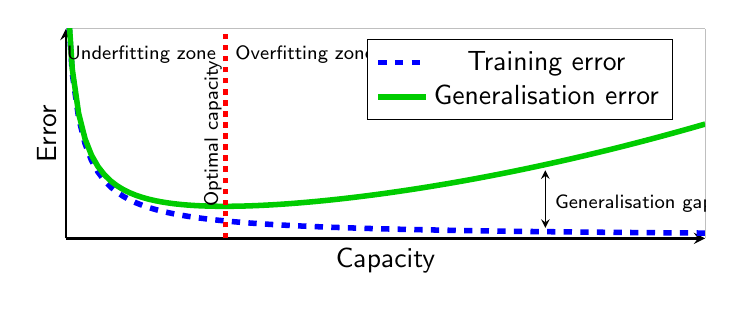
\begin{tikzpicture}[font=\sffamily\sansmath]

    \begin{axis}
        [
        xmin=0,
        xmax=2,
        ymin=0,
        ymax=2,
        xlabel=Capacity,
        ylabel=Error,
        ticks=none,
        xtick={2},
        ytick={2},
        xticklabels={\empty},
        yticklabels={\empty},
        ymajorgrids=true,
        xmajorgrids=true,
        width=0.8\linewidth,
        height=0.35\linewidth,
        axis line style = thick,
        legend style={at={(0.95,0.95)},anchor=north east}
        ]
        \addplot[domain=0.00:2.0, blue, dashed] {0.25/(3*x+0.1) + 0.01};   % Training error
        \addlegendentry{Training error}
        \addplot[domain=0.00:2.0, green!80!black] {0.25/(3*x+0.1) + 0.1*x + 0.2 *x*x + 0.05};  % Generalisation error
        \addlegendentry{Generalisation error}
%      \addplot[domain=0.39:1.61,black] {3*(x-2)*x+3.8};  %Total error
        \addplot[dotted, red] coordinates {(0.5,0) (0.5,2)};           %Optimum model complexity
        \addplot[thin, <->] coordinates {(1.5,0.1) (1.5,0.65)};       %Optimum model complexity

        \node[OptimumStyle] at (axis cs:0.46,1.0) {Optimal capacity};
        \node[UnderfitStyle] at (axis cs:0.5,1.75) {Underfitting zone};
        \node[OverfitStyle] at (axis cs:0.5,1.75) {Overfitting zone};
        \node[OverfitStyle] at (axis cs:1.5,0.33) {Generalisation gap};
%      \node[anchor=south west,text=Maroon] at (axis cs:1.4,0.4){Bias\textsuperscript{2}};
%      \node[anchor=north west,text=TealBlue] at (axis cs:1.4,0.85){Variance};
%      \node[anchor=south east,align=center] at (axis cs:1.5,1.5){Total\\error};
%        \legend{}
    \end{axis}
\end{tikzpicture}
%}

%\end{document}
    \captionsetup{format=hang} % hanging captions
    \caption{
        Typical relationship between capacity and error. Training and test error
        behave differently. At the left end of the graph, training error and
        generalization error are both high. This is the \textbf{underfitting
        regime} As we increase capacity, training error decreases, but the gap
        between training and generalisation error increases. Eventually, the
        size of this gap outweighs the decrease in training error, and we enter
        the \textbf{overfitting regime}, where capacity is too large, above the
        \textbf{optimal capacity}. Adapted from Goodfellow et al.
        \cite{Goodfellow-et-al-2016}.
    }
    \label{fig:capacity}
\end{figure}

\subsubsection{No Free Lunch Theorem}
%%%%%%%%%%%%%%%%%%%%%%%%%%%%%%%%%%%%%%%%%%%%%%%%%%%%%%%%%%%%%%%%%%%%%%%%%%%%%%%%

The \gls{NFLT}, sometimes abbreviated as \gls{NFL}, is a simple but important
concept in \gls{ML} and optimisation~\cite{Wolpert1997}. The theorem suggests
that an optimisation technique will perform equally well as any other when
averaging its performance over the set of all possible problems. This implies
that there is no single best technique for addressing an arbitrary problem. Luke
states the following in \textit{essentials of
metaheuristics}~\cite{luke2012essentials}:

\begin{fancyquotes}
    The \gls{NFL} stated that within certain constraints, over the space of
    all possible problems, every optimization technique will perform as well as
    every other one on average (including Random Search)
\end{fancyquotes}

This argues that without having substantive information about the fundamentals
of the problem being modelled, choosing to apply a single technique to an
arbitrary problem will not yield a predictably better or worse result than
applying another to the same problem. Therefore, in the case where the
underlying process being optimised is not well-understood, a variety of
techniques should be applied.

However, in practice, knowledge to some degree is known about the problem which
is being optimised, or to which a learning algorithm is being applied. This
theorem highlights the importance of having a clear understanding of the problem
at hand before applying a learning algorithm or an optimisation technique.
Domingos states ~\cite{Domingos15}:

\begin{fancyquotes}
    In the meantime, the practical consequence of the “no free lunch”
    theorem is that there’s no such thing as learning without knowledge. Data
    alone is not enough.
\end{fancyquotes}

This theorem, in effect, motivates the true goal of machine learning, as worded
by Goodfellow et al.~\cite[p.~116]{Goodfellow-et-al-2016}:

\begin{fancyquotes}
    This means that the goal of machine learning research is not to seek
    a universal learning algorithm or the absolute best learning algorithm.
    Instead, our goal is to understand what kinds of distributions are relevant
    to the “real world” that an AI agent experiences, and what kinds of machine
    learning algorithms perform well on data drawn from the kinds of
    data-generating distributions we care about.
\end{fancyquotes}


This is an important insight and directly relates to a learning algorithm's
tendency to overfit or underfit. If we do not have a clear understanding of the
level of complexity of the task we are trying to find a solution to with our
learning algorithm, then we are likely to overfit or underfit. If one assumes
the complexity of the problem to be higher than its true complexity, the learner
will have access to a much larger hypothesis space (capacity) than what is
optimal. On the other hand, if we underestimate the complexity, it is almost
certain that we will design an algorithm with insufficient capacity. This also
extends to the quantity and quality of training data that we are training with.
It is impossible, for example, to model an $n^\text{th}$ order process with anything less
than $n$ training samples without underfitting, and this is without considering
the possibility of measurement noise.

\subsubsection{Regularization}
%%%%%%%%%%%%%%%%%%%%%%%%%%%%%%%%%%%%%%%%%%%%%%%%%%%%%%%%%%%%%%%%%%%%%%%%%%%%%%%%
Generally speaking, regularization is any modification we make to a learning
algorithm that is intended to reduce its generalisation error but not its
training error. Due to the large number of techniques that fit this description
within \gls{ML} and its subfields, it is outside the scope of this paper to
exhaustively cover this concept, however the core idea behind regularization
within \gls{ML} is motivated here through one of its earliest forms.

A fundamental approach to regularization in \gls{ML} originating
from \textit{statistical learning} is the use of \textbf{parameter norm
penalties} which aim at guiding the parameter vectors through the addition of a
penalty term in the objective (cost/loss) function being minimised. This penalty
constrains (regularizes) or shrinks the optimal \gls{w_vec} estimate towards
zero, effectively discouraging a learning algorithm from producing an
excessively complex model, to avoid overfitting. Norm penalty methods can be
generalized as:

\begin{equation}
    \gls{J_reg}(\gls{m_theta}; \gls{X}, \gls{Y})
    =
    \gls{J}(\gls{m_theta}; \gls{X}, \gls{Y})_\text{train}
    +
    \gls{w_reg}\gls{o_reg}({\gls{m_theta}}),
    \label{eq:norm_penalty_reg}
\end{equation}
\begin{equation*}
    \begin{aligned}
        \textrm{where, }
        \eqdesc{J_reg}\text{,} \\
        \eqdesc{m_theta}\text{,} \\
        \eqdesc{X}\text{,} \\
        \eqdesc{Y}\text{,} \\
        \eqdesc{J}\text{,} \\
        \eqdesc{w_reg}\text{,} \\
        \eqdesc{o_reg}\text{.} \\
    \end{aligned}
\end{equation*}

For learning algorithms which make use of gradient-based learning techniques,
the parameter gradient must be computed. This can be challenging to compute in
cases where the derivative of a cost function is not easily determined, such as
with \gls{MAE} defined by \autoref{eq:MAE}. The expression of the regularized
cost function is given by,

\begin{equation}
    \nabla_{\gls{w_vec}}\gls{J_reg}(\gls{w_vec};\gls{X},\gls{Y})
    =
    \nabla_{\gls{w_vec}}\gls{J}(\gls{w_vec};\gls{X},\gls{Y})
    +
    \gls{w_reg}\nabla_{\gls{w_vec}}\gls{o_reg}(\gls{m_theta})\text{.}
    \label{eq:norm_penalty_reg_graident}
\end{equation}

$\bm{\text{L}^2}$ \textbf{regularization}, also known as \textbf{ridge
regression}, \textbf{weight decay} or \textbf{Tikhonov regularization}
\cite[p.~227]{Goodfellow-et-al-2016}, is a parameter norm regularization method
which drives the weights of a model towards the origin in the weight space and
contributes to \autoref{eq:norm_penalty_reg} as,
\begin{equation}
    \gls{o_reg}(\gls{m_theta})=\frac{1}{2}||\gls{w_vec}||^2_2.
    \label{eq:l2_reg}
\end{equation}

Weight decay suppresses any irrelevant components of the weight vector by
choosing the smallest vector that solves the learning problem. Furthermore if
the weight decay parameter is chosen correctly, noise may be suppressed in the
output, subsequently improving generalization~\cite{NIPS1991_8eefcfdf}.

$\bm{\text{L}^1}$ \textbf{regularization}, also known as \textbf{\gls{LASSO}
regression} is a parameter norm regularization method which penalizes the
largest weight magnitudes in the weight vector. It is defined by,
\begin{equation}
    \gls{o_reg}(\gls{m_theta})=||\gls{w_vec}||_1.
    \label{eq:l1_reg}
\end{equation}

\begin{figure}[!htp]
    \centering
    \begin{subfigure}[b]{0.49\textwidth}
        \centering
        % MIT License
%
% Copyright (c) 2021 Geoffrey H. Garrett
%
% Permission is hereby granted, free of charge, to any person obtaining a copy
% of this software and associated documentation files (the "Software"), to deal
% in the Software without restriction, including without limitation the rights
% to use, copy, modify, merge, publish, distribute, sublicense, and/or sell
% copies of the Software, and to permit persons to whom the Software is
% furnished to do so, subject to the following conditions:
%
% The above copyright notice and this permission notice shall be included in all
% copies or substantial portions of the Software.
%
% THE SOFTWARE IS PROVIDED "AS IS", WITHOUT WARRANTY OF ANY KIND, EXPRESS OR
% IMPLIED, INCLUDING BUT NOT LIMITED TO THE WARRANTIES OF MERCHANTABILITY,
% FITNESS FOR A PARTICULAR PURPOSE AND NONINFRINGEMENT. IN NO EVENT SHALL THE
% AUTHORS OR COPYRIGHT HOLDERS BE LIABLE FOR ANY CLAIM, DAMAGES OR OTHER
% LIABILITY, WHETHER IN AN ACTION OF CONTRACT, TORT OR OTHERWISE, ARISING FROM,
% OUT OF OR IN CONNECTION WITH THE SOFTWARE OR THE USE OR OTHER DEALINGS IN THE
% SOFTWARE.

%%%%%%%%%%%%%%%%%%%%%%%%%%%%%%%%%%%%%%%%%%%%%%%%%%%%%%%%%%%%%%%%%%%%%%%%%%%%%%%
% ACKNOWLEDGEMENTS
%%%%%%%%%%%%%%%%%%%%%%%%%%%%%%%%%%%%%%%%%%%%%%%%%%%%%%%%%%%%%%%%%%%%%%%%%%%%%%%
% Design and implementation of this diagram was inspired and adapted from:
% https://tex.stackexchange.com/questions/573127/tikz-plots-are-not-centered

%%%%%%%%%%%%%%%%%%%%%%%%%%%%%%%%%%%%%%%%%%%%%%%%%%%%%%%%%%%%%%%%%%%%%%%%%%%%%%%
% DEPENDENCIES
%%%%%%%%%%%%%%%%%%%%%%%%%%%%%%%%%%%%%%%%%%%%%%%%%%%%%%%%%%%%%%%%%%%%%%%%%%%%%%%
%\usepackage{tikz}
%\usepackage{amsmath}
%\usetikzlibrary{shapes.geometry}

%%%%%%%%%%%%%%%%%%%%%%%%%%%%%%%%%%%%%%%%%%%%%%%%%%%%%%%%%%%%%%%%%%%%%%%%%%%%%%%
% USER STYLING
%%%%%%%%%%%%%%%%%%%%%%%%%%%%%%%%%%%%%%%%%%%%%%%%%%%%%%%%%%%%%%%%%%%%%%%%%%%%%%%

%\begin{tikzpicture}
%    \begin{axis}[
%        xmin=-4,
%        xmax=4.5,
%        ymin=-0.5,
%        ymax=3.5,
%        ticks=none,
%        xticklabels={\empty},
%        yticklabels={\empty},
%        ymajorgrids=false,
%        xmajorgrids=false,
%        axis line style = semithick,
%        axis equal image,
%%        width=1.2\columnwidth
%    ]
%    \draw (axis cs:0,3) circle [blue, radius=1];
%    \end{axis}
%\end{tikzpicture}


\newcommand{\plotregularizercontour}[2] {
    \addplot[dashed, dash phase=0.1em, color=none, draw opacity=1, mark=none, fill=cyan!20, fill opacity=0.4] coordinates {
        (#1, 0)
        (0, -#1)
        (-#1, 0)
        (0, #1)
        (#1, 0)
    };
}
%    \draw[dashed, dash phase=0.1em, fill=cyan!20, fill opacity=0.5] (axis cs:0,0) circle [#2, radius=#1];

\newcommand{\plotobjectivecontour}[6] {
    \draw[#6, thin] (#1, #2) ellipse[x radius=#3, y radius=#4, rotate=#5, dashed]; % <---
}

\begin{tikzpicture}

    \begin{axis}
        [
        xticklabels={\empty},
        yticklabels={\empty},
        xlabel={$w_1$},
        ylabel={$w_2$},
        ymajorgrids=false,
        xmajorgrids=false,
        axis line style = semithick,
        ymin=-3.6, ymax=9.5,
        xmin=-3.6, xmax=9.5,
        axis lines=middle,
        axis equal image,
        yticklabels={$a$},
        ]

        % some constants
        \def\ex{4};
        \def\ey{5.95};
        \def\rot{-60};
        \def\ext{3.5};

        % regularizer contour
        \plotregularizercontour{3.5}{}
        \plotregularizercontour{2.5}{}
        \plotregularizercontour{1.5}{}
        \plotregularizercontour{0.5}{}

        % \tilde{w}
        \addplot[color=black, draw opacity=1, mark=*] coordinates {(0, \ext)};
        \node[anchor=east] at (0, \ext) {$\tilde{\bm{w}}$}; % <---

        % J contour
        \plotobjectivecontour{\ex}{\ey}{1.0cm}{2.0cm}{\rot}{red}
        \plotobjectivecontour{\ex}{\ey}{0.8cm}{1.8cm}{\rot}{red!50!orange}
        \plotobjectivecontour{\ex}{\ey}{0.6cm}{1.6cm}{\rot}{red!20!orange}
        \plotobjectivecontour{\ex}{\ey}{0.4cm}{1.4cm}{\rot}{orange!50!green}
        \node[] at (\ex, \ey) {$\bm{w}^*$}; % <---
    \end{axis}
\end{tikzpicture}
        \subcaption{$\text{L}^1~\text{regularization}$}
        \label{fig:underfitting}
    \end{subfigure}\hfil
    \begin{subfigure}[b]{0.49\textwidth}
        \centering
        % MIT License
%
% Copyright (c) 2021 Geoffrey H. Garrett
%
% Permission is hereby granted, free of charge, to any person obtaining a copy
% of this software and associated documentation files (the "Software"), to deal
% in the Software without restriction, including without limitation the rights
% to use, copy, modify, merge, publish, distribute, sublicense, and/or sell
% copies of the Software, and to permit persons to whom the Software is
% furnished to do so, subject to the following conditions:
%
% The above copyright notice and this permission notice shall be included in all
% copies or substantial portions of the Software.
%
% THE SOFTWARE IS PROVIDED "AS IS", WITHOUT WARRANTY OF ANY KIND, EXPRESS OR
% IMPLIED, INCLUDING BUT NOT LIMITED TO THE WARRANTIES OF MERCHANTABILITY,
% FITNESS FOR A PARTICULAR PURPOSE AND NONINFRINGEMENT. IN NO EVENT SHALL THE
% AUTHORS OR COPYRIGHT HOLDERS BE LIABLE FOR ANY CLAIM, DAMAGES OR OTHER
% LIABILITY, WHETHER IN AN ACTION OF CONTRACT, TORT OR OTHERWISE, ARISING FROM,
% OUT OF OR IN CONNECTION WITH THE SOFTWARE OR THE USE OR OTHER DEALINGS IN THE
% SOFTWARE.

%%%%%%%%%%%%%%%%%%%%%%%%%%%%%%%%%%%%%%%%%%%%%%%%%%%%%%%%%%%%%%%%%%%%%%%%%%%%%%%
% ACKNOWLEDGEMENTS
%%%%%%%%%%%%%%%%%%%%%%%%%%%%%%%%%%%%%%%%%%%%%%%%%%%%%%%%%%%%%%%%%%%%%%%%%%%%%%%
% Design and implementation of this diagram was inspired and adapted from:
% https://tex.stackexchange.com/questions/573127/tikz-plots-are-not-centered

%%%%%%%%%%%%%%%%%%%%%%%%%%%%%%%%%%%%%%%%%%%%%%%%%%%%%%%%%%%%%%%%%%%%%%%%%%%%%%%
% DEPENDENCIES
%%%%%%%%%%%%%%%%%%%%%%%%%%%%%%%%%%%%%%%%%%%%%%%%%%%%%%%%%%%%%%%%%%%%%%%%%%%%%%%
%\usepackage{tikz}
%\usepackage{amsmath}

%%%%%%%%%%%%%%%%%%%%%%%%%%%%%%%%%%%%%%%%%%%%%%%%%%%%%%%%%%%%%%%%%%%%%%%%%%%%%%%
% USER STYLING
%%%%%%%%%%%%%%%%%%%%%%%%%%%%%%%%%%%%%%%%%%%%%%%%%%%%%%%%%%%%%%%%%%%%%%%%%%%%%%%

%\begin{tikzpicture}
%    \begin{axis}[
%        xmin=-4,
%        xmax=4.5,
%        ymin=-0.5,
%        ymax=3.5,
%        ticks=none,
%        xticklabels={\empty},
%        yticklabels={\empty},
%        ymajorgrids=false,
%        xmajorgrids=false,
%        axis line style = semithick,
%        axis equal image,
%%        width=1.2\columnwidth
%    ]
%    \draw (axis cs:0,3) circle [blue, radius=1];
%    \end{axis}
%\end{tikzpicture}


\newcommand{\plotregularizercontour}[2] {
%        \addplot[dashed, dash phase=0.1em, thick, color=#2, draw opacity=1, mark=none, fill=#2, fill opacity=0.01] coordinates {
%            (#1, 0)
%            (0, -#1)
%            (-#1, 0)
%            (0, #1)
%            (#1, 0)
%        };
    \draw[dashed, dash phase=0.1em, fill=cyan!20, fill opacity=0.4] (axis cs:0,0) circle [#2, radius=#1];

}

\newcommand{\plotobjectivecontour}[6] {
    \draw[#6, thin] (#1, #2) ellipse[x radius=#3, y radius=#4, rotate=#5, dashed]; % <---
}

\begin{tikzpicture}

    \begin{axis}
        [
        xticklabels={\empty},
        yticklabels={\empty},
        xlabel={$w_1$},
        ylabel={$w_2$},
        ymajorgrids=false,
        xmajorgrids=false,
        axis line style = semithick,
        ymin=-3.5, ymax=9.5,
        xmin=-3.5, xmax=9.5,
        axis lines=middle,
        axis equal image,
%        xtick=\empty,
%        ytick={4},
        yticklabels={$a$},
        ]
        \def\ex{4};
        \def\ey{5.95};
        \def\rot{-60};

        \plotregularizercontour{3.9em}{}
        \plotregularizercontour{2.9em}{}
        \plotregularizercontour{1.9em}{}
        \plotregularizercontour{0.9em}{}

        % J contour
        \plotobjectivecontour{\ex}{\ey}{1.0cm}{2.0cm}{\rot}{red}
        \plotobjectivecontour{\ex}{\ey}{0.8cm}{1.8cm}{\rot}{red!50!orange}
        \plotobjectivecontour{\ex}{\ey}{0.6cm}{1.6cm}{\rot}{red!20!orange}
        \plotobjectivecontour{\ex}{\ey}{0.4cm}{1.4cm}{\rot}{orange!50!green}
        \node[] at (\ex, \ey) {$\bm{w}^*$}; % <---

        % \tilde{w}
        \addplot[color=black, draw opacity=1, mark=*] coordinates {(0.9,3)};
        \node[anchor=north east, shape=circle, fill=white, fill opacity=0.0, text opacity=1] at (0.9,3.2) {$\tilde{\bm{w}}$}; % <---

    \end{axis}
\end{tikzpicture}
        \subcaption{$\text{L}^2~\text{regularization}$}
        \label{fig:underfitting}
    \end{subfigure}\hfil
    \captionsetup{format=hang} % hanging captions
    \caption{
        An illustration of the effect of of (a) L$^1$ and (b) L$^2$ (or weight
        decay) regularization on the optimal value of \gls{w_vec} for
        $\gls{w_vec}\in\mathbb{R}^2$. The solid contours show equal values of
        the unregularized objective. The dashed contours show equal values of
        the respective norm regularizer. The point $\tilde{\bm{w}}$ shows these
        competing objectives reach an equilibrium, determined by the
        minimization of \autoref{eq:norm_penalty_reg}, with each norm's
        regularizer substituted, \autoref{eq:l1_reg} and  \autoref{eq:l2_reg}
        respectively. Illustration adapted from Goodfellow et al.~\cite[p.~116]{Goodfellow-et-al-2016}
        and Hastie et al.~\cite[p.~71]{hastie2009elements}
    }
    \label{fig:l1-l2-regularization}
\end{figure}

\textbf{Elastic net regularization} is a combination of both $L^1$ and $L^2$
regularization was introduced by Zou and Hastie \cite{ZouHastie2005} and is
expressed by:
\begin{equation}
    \gls{o_reg}(\gls{m_theta})=\frac{1-\gls{b_ela}}{2}||\gls{w_vec}||^2_2 + \gls{b_ela}||\gls{w_vec}||_1\text{,}
\end{equation}
\begin{equation*}
    \begin{aligned}
        \textrm{where, }
        \eqdesc{b_ela}\text{.} \\
    \end{aligned}
\end{equation*}

Looking again at \autoref{fig:l1-l2-regularization}, one might wonder if an
alternative vector norm regularization method would be more appropriate. Hastie
et al. state that experience suggests that it is not worth the extra variance
incurred to estimate what vector norm $L^p$ should be used based on the
data~\cite[p.~73]{hastie2009elements}.
%Given some function $f(\gls{x_in};\gls{m_theta})$ being learnt
%by being modelled by a learning algorithm,

\subsection{Hyperparameters and Validation Sets}
%%%%%%%%%%%%%%%%%%%%%%%%%%%%%%%%%%%%%%%%%%%%%%%%%%%%%%%%%%%%%%%%%%%%%%%%%%%%%%%%
Most machine learning algorithms have parameters referred to as hyperparameters.
These define some algorithm setting which are not adapted by the algorithm
itself during learning. This however does not mean that the algorithm cannot
exist in a subroutine during which the hyperparameters are optimised. An example
of a hyperaparameter is the value of \gls{w_reg} chosen in
\autoref{eq:norm_penalty_reg}. This parameter is kept constant throughout the
learning algorithm and heavily influences the resultant model. Optimizing
hyperparameters on the training set that control capacity is generally not
appropriated. This is because the hyperparameter would tend to towards
overfitting the training data, which would result in the best test score, but
with high variance and thus poor generalization on unseen data. Therefore as
mentioned, the training procedure can be used as a subroutine of a larger
optimization problem, which uses a validation set to assess performance of the
hyperparameters of the model.

\begin{figure}[htp]
    \centering
    % MIT License
%
% Copyright (c) 2021 Geoffrey H. Garrett
%
% Permission is hereby granted, free of charge, to any person obtaining a copy
% of this software and associated documentation files (the "Software"), to deal
% in the Software without restriction, including without limitation the rights
% to use, copy, modify, merge, publish, distribute, sublicense, and/or sell
% copies of the Software, and to permit persons to whom the Software is
% furnished to do so, subject to the following conditions:
%
% The above copyright notice and this permission notice shall be included in all
% copies or substantial portions of the Software.
%
% THE SOFTWARE IS PROVIDED "AS IS", WITHOUT WARRANTY OF ANY KIND, EXPRESS OR
% IMPLIED, INCLUDING BUT NOT LIMITED TO THE WARRANTIES OF MERCHANTABILITY,
% FITNESS FOR A PARTICULAR PURPOSE AND NONINFRINGEMENT. IN NO EVENT SHALL THE
% AUTHORS OR COPYRIGHT HOLDERS BE LIABLE FOR ANY CLAIM, DAMAGES OR OTHER
% LIABILITY, WHETHER IN AN ACTION OF CONTRACT, TORT OR OTHERWISE, ARISING FROM,
% OUT OF OR IN CONNECTION WITH THE SOFTWARE OR THE USE OR OTHER DEALINGS IN THE
% SOFTWARE.

%%%%%%%%%%%%%%%%%%%%%%%%%%%%%%%%%%%%%%%%%%%%%%%%%%%%%%%%%%%%%%%%%%%%%%%%%%%%%%%
% ACKNOWLEDGEMENTS
%%%%%%%%%%%%%%%%%%%%%%%%%%%%%%%%%%%%%%%%%%%%%%%%%%%%%%%%%%%%%%%%%%%%%%%%%%%%%%%
% Design and implementation of this diagram was inspired and adapted from:
% https://tex.stackexchange.com/questions/573127/tikz-plots-are-not-centered

%%%%%%%%%%%%%%%%%%%%%%%%%%%%%%%%%%%%%%%%%%%%%%%%%%%%%%%%%%%%%%%%%%%%%%%%%%%%%%%
% DEPENDENCIES
%%%%%%%%%%%%%%%%%%%%%%%%%%%%%%%%%%%%%%%%%%%%%%%%%%%%%%%%%%%%%%%%%%%%%%%%%%%%%%%
%\usepackage{tikz}
% \usetikzlibrary{positioning, decorations.text, calc}

%%%%%%%%%%%%%%%%%%%%%%%%%%%%%%%%%%%%%%%%%%%%%%%%%%%%%%%%%%%%%%%%%%%%%%%%%%%%%%%
% USER STYLING
%%%%%%%%%%%%%%%%%%%%%%%%%%%%%%%%%%%%%%%%%%%%%%%%%%%%%%%%%%%%%%%%%%%%%%%%%%%%%%%


%

%\tikzset{declare function={f(\x)=(-0.06*(\x-2)+0.5)*(\x-2)*(\x-2);}}% applied math style
%\foreach \Z in {1,...,42} {\pgfmathsetmacro{\X}{\Z/10}%
%\pgfmathsetmacro{\Y}{f(\X)+0.9*rnd}%
%\ifnum\Z=1
%\xdef\LstOne{(\X,\Y)}%
%\xdef\LstTwo{"(\X,\Y)"}%
%\else
%\xdef\LstOne{\LstOne (\X,\Y)}%
%\xdef\LstTwo{\LstTwo,"(\X,\Y)"}%
%\fi}%

\newcommand{\plotobservations} {
    \addplot[only marks, draw=blue, fill=blue] coordinates {
        (0.0, 2.5991314214589614)
        (0.4444444444444444, 1.3463852235976501)
        (0.8888888888888888, 1.3558966978583558)
        (1.3333333333333333, 0.1719351250071693)
        (1.7777777777777777, 0.0549444514647925)
        (2.2222222222222223, 0.45130282341732175)
        (2.6666666666666665, -0.04104830486674099)
        (3.1111111111111107, 0.3752375262271346)
        (3.5555555555555554, 1.034685792786699)
        (4.0, 1.430935111399573)
    };
}

\newcommand{\plottruedistribution}{
    \addplot[domain=-0.5:4.5, dashed, thin, gray!75] {
        (-0.06 * (x - 2) + 0.5) * (x - 2) * (x - 2)
    };


}

%%%%%%%%%%%%%%%%%%%%%%%%%%%%%%%%%%%%%%%%%%%%%%%%%%%%%%%%%%%%%%%%%%%%%%%%%%%%%%%%
\begin{subfigure}[b]{0.32\textwidth}
    \centering
    \begin{tikzpicture}
        \begin{axis}[
            xmin=-0.5,
            xmax=4.5,
            ymin=-0.5,
            ymax=3.5,
            ticks=none,
            xticklabels={\empty},
            yticklabels={\empty},
            ymajorgrids=false,
            xmajorgrids=false,
            axis line style = semithick,
            width=1.2\columnwidth]
            \plotobservations
            \plottruedistribution
            \addplot[domain=-0.5:4.5, thick, green!50!black] {
                1.3645283299815407 - 0.24329387 * x
            };
        \end{axis}
    \end{tikzpicture}
    \subcaption{Underfitting (Excessive $\alpha$)}
    \label{fig:ref-underfitting}
\end{subfigure}\hfil
%%%%%%%%%%%%%%%%%%%%%%%%%%%%%%%%%%%%%%%%%%%%%%%%%%%%%%%%%%%%%%%%%%%%%%%%%%%
\begin{subfigure}[b]{0.32\textwidth}
    \centering
    \begin{tikzpicture}
        \begin{axis}[
            xmin=-0.5,
            xmax=4.5,
            ymin=-0.5,
            ymax=3.5,
            ticks=none,
            xticklabels={\empty},
            yticklabels={\empty},
            ymajorgrids=false,
            xmajorgrids=false,
            axis line style = semithick,
            width=1.2\columnwidth]
            \plotobservations
            \plottruedistribution
            \addplot[domain=-0.5:4.5, thick, green!50!black] {
                + 2.5332784046893866
                - 2.31697944 * x
                + 0.58870681 * x ^ 2
                - 0.01887639 * x ^ 3
            };
        \end{axis}
    \end{tikzpicture}
    \subcaption{Appropriate (Medium $\alpha$)}
    \label{fig:reg-appropriate-capacity}
\end{subfigure}\hfil
%%%%%%%%%%%%%%%%%%%%%%%%%%%%%%%%%%%%%%%%%%%%%%%%%%%%%%%%%%%%%%%%%%%%%%%%%%%%%%%%%%%
\begin{subfigure}[b]{0.32\textwidth}
    \centering
    \begin{tikzpicture}
        \begin{axis}[
            xmin=-0.5,
            xmax=4.5,
            ymin=-0.5,
            ymax=3.5,
            ticks=none,
            xticklabels={\empty},
            yticklabels={\empty},
            ymajorgrids=false,
            xmajorgrids=false,
            samples=200,
            axis line style = semithick,
            width=1.2\columnwidth]
            \plotobservations
            \plottruedistribution
            \addplot[domain=-0.5:4.5, thick, green!50!black] {
                +2.599131312448361
                -10.588139742958015 * x^1
                +25.074367329152583 * x^2
                -12.832852119149837 * x^3
                -15.29078616509039 * x^4
                +10.350960340047243 * x^5
                +10.94777207200677 * x^6
                -14.543216443491573 * x^7
                +6.786937457668481 * x^8
                -1.5968672908165933 * x^9
                +0.18962693236609746 * x^10
                -0.009014002246939552 * x^11
            };
        \end{axis}
    \end{tikzpicture}
    \subcaption{Overfitting ($\alpha\rightarrow{0}$)}
    \label{fig:overfitting}
\end{subfigure}

    \captionsetup{format=hang} % hanging captions
    \caption{
        Regression modelling, as performed in \autoref{fig:capacity-plots}. The
        effect of varying the regularization coefficient \gls{w_reg} in
        \autoref{eq:norm_penalty_reg} is shown in the left panel. The effect of
        varying the regularization coefficient \gls{w_reg} in
        \autoref{eq:l1_reg} is shown in the right panel. The effect of varying
        the regularization coefficient \gls{w_reg} in \autoref{eq:l2_reg} is
        depicted in relation to its effect on the capacity of the model. (a)
        shows that \gls{w_ref} has been chosen excessively, causing the
        hypothesis space available to the learner to be insufficient. (b) shows
        that \gls{w_ref} has been chosen appropriately, resulting in a model
        that generalizes well, and captures the true distribution being learnt.
        (c) shows that no regularization has occurred, resulting in a model that
        overfits the noisy data.
    }
    \label{fig:reg-capacity-plots}
\end{figure}

The importance of optimizing the hyperparameters of a learning algorithm,
especially relating to capacity, are illustrated in
\autoref{fig:reg-capacity-plots} using the example of regularization weight
$\gls{w_reg}$.

\subsubsection{The bias-variance tradeoff}
Bias and variance measure two different sources in an estimator (model).
\textbf{The bias-variance tradeoff} is an inherent property of a model which
allows for the variance of the estimated parameter to be reduced by increasing
the bias of the model and vice versa. This property naturally presents the
\textbf{bias-variance dilemma} or \textbf{bias-variance problem}, which is the
conflict present in a supervised learning algorithm when it attempts to
generalize to new data outside of the training dataset. The most common way to
address this problem is through cross-validation. Alternatively the estimates
of the model parameters $\hat{\theta}_m$ can be compared using \gls{MSE}.

\begin{equation}
    \begin{aligned}
        \text{\gls{MSE}}&=\gls{E}[(\hat{\theta}_m-\theta)^2]\\
        &=\text{Bias}(\hat{\theta}_m)^2+\text{Var}(\hat{\theta}_m)
    \end{aligned}
\end{equation}

This concept of the bias-variance tradeoff is highly coupled to the concepts of
capacity, underfitting and overfitting as evident in
\autoref{fig:bias-variance}.

\begin{figure}[htp!]
    \centering
    % Adapted from https://raw.githubusercontent.com/MartinThoma/LaTeX-examples/master/tikz/bias-variance/bias-variance.tex

%\usetikzlibrary{arrows.meta,bending}
\tikzset{>=stealth,
    OptimumStyle/.style={align=center,anchor=center,rotate=90,font=\sffamily\scriptsize},
    OverfitStyle/.style={align=center,anchor=west,rotate=0,font=\sffamily\scriptsize},
    UnderfitStyle/.style={align=center,anchor=east,rotate=0,font=\sffamily\scriptsize},
}
%\pgfplotsset{compat=1.17,
%    samples=101,
%    axis lines = left,
%    every axis plot/.append style={line width=2pt},
%}

%\begin{document}
%\fbox{
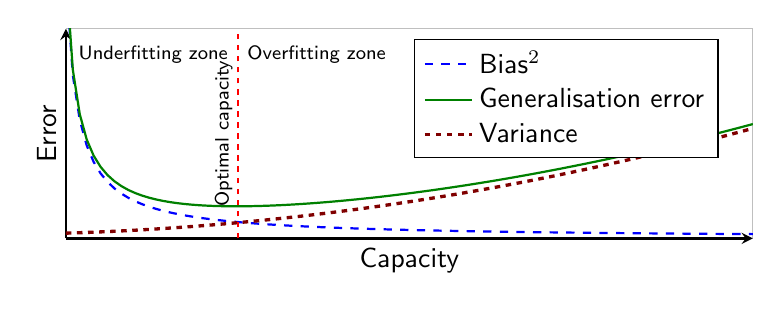
\begin{tikzpicture}[font=\sffamily\sansmath]

    \begin{axis}
        [
        xmin=0,
        xmax=2,
        ymin=0,
        ymax=2,
        xlabel=Capacity,
        ylabel=Error,
        ticks=none,
        xtick={2},
        ytick={2},
        xticklabels={\empty},
        yticklabels={\empty},
        ymajorgrids=true,
        xmajorgrids=true,
        samples=100,
        width=0.85\linewidth,
        height=0.35\linewidth,
        axis line style = thick,
        legend cell align={left},
        legend style={at={(0.95,0.95)},anchor=north east}
        ]
        \addplot[domain=0.00:2.0, blue, dashed, thick] {0.25/(3*x+0.1)};   % Error due to bias
        \addlegendentry{Bias$^2$}
        \addplot[domain=0.00:2.0, green!50!black, thick] {0.25/(3*x+0.1) + 0.1*x + 0.2 *x*x + 0.05};  % Generalisation error
        \addlegendentry{Generalisation error}
        \addplot[domain=0.00:2.0, red!50!black, dotted, very thick] {0.1*x + 0.2 *x*x + 0.05};  % Error due to variance
        \addlegendentry{Variance}
%      \addplot[domain=0.39:1.61,black] {3*(x-2)*x+3.8};  %Total error
        \addplot[dotted, red, thick] coordinates {(0.5,0) (0.5,2)};           %Optimum model complexity
%        \addplot[thin, <->] coordinates {(1.5,0.1) (1.5,0.65)};       %Optimum model complexity

        \node[OptimumStyle] at (axis cs:0.46,1.0) {Optimal capacity};
        \node[UnderfitStyle] at (axis cs:0.5,1.75) {Underfitting zone};
        \node[OverfitStyle] at (axis cs:0.5,1.75) {Overfitting zone};
%        \node[OverfitStyle] at (axis cs:1.5,0.33) {Generalisation gap};
%      \node[anchor=south west,text=Maroon] at (axis cs:1.4,0.4){Bias\textsuperscript{2}};
%      \node[anchor=north west,text=TealBlue] at (axis cs:1.4,0.85){Variance};
%      \node[anchor=south east,align=center] at (axis cs:1.5,1.5){Total\\error};
%        \legend{}
    \end{axis}
\end{tikzpicture}
%}

%\end{document}
    \captionsetup{format=hang} % hanging captions
    \caption{
        The error source of a model evaluated using \gls{MSE}. As the capacity of
        a model increases, the error source of the model transitions from bias
        dominated to variance dominated. The sum of both error sources yields
        the generalization error which is U-shaped. The optimal capacity of the
        model is exactly at this transition, where the bias error intersects the
        variance error. To the right of the transition, the model is overfitting
        and to the left, underfitting. This relationship is similar to that seen
        in \autoref{fig:capacity}.
    }
    \label{fig:bias-variance}
\end{figure}

%\subsubsection{Resubstitution}
%%%%%%%%%%%%%%%%%%%%%%%%%%%%%%%%%%%%%%%%%%%%%%%%%%%%%%%%%%%%%%%%%%%%%%%%%%%%%%%%

%\subsubsection{Holdout}
%%%%%%%%%%%%%%%%%%%%%%%%%%%%%%%%%%%%%%%%%%%%%%%%%%%%%%%%%%%%%%%%%%%%%%%%%%%%%%%%

\subsubsection{Cross-Validation}
%%%%%%%%%%%%%%%%%%%%%%%%%%%%%%%%%%%%%%%%%%%%%%%%%%%%%%%%%%%%%%%%%%%%%%%%%%%%%%%%
Cross-validation is often used for the assessment and optimization of
hyperparameters which improve a learning algorithm's ability to generalize on
unseen data. This is achieved through the separation of training folds from a
validation fold. The training fold is then separated into training data and
test data, while the validation fold is left out of the training procedure
entirely. The validation fold is then used to assess the performance of the
model on unseen data which has not been used to obtain the estimates of the
model parameters. A common way of performing cross-validation is to use a
\gls{KFCV}, where $k$ is the number of \textit{approximately
equal} folds that the data is separated into. The total dataset is then iterated
through, where each fold is used once as the validation fold and the remaining
folds are used as the training folds. The validation error is then calculated by
averaging the errors of all iterations. This is depicted in
\autoref{fig:kfold-cv}. \cite[p.~241-245]{hastie2009elements}


\begin{figure}[htbp]
    \centering
    % DEP
% \usetikzlibrary{matrix}

% ACK
% https://tex.stackexchange.com/questions/429451/k-fold-cross-validation-figure-using-tikz-or-table

\begin{tikzpicture}
    \matrix (M)
        [
        matrix of nodes,
        nodes={
            minimum height = 6mm,
            minimum width = 1.3cm,
            outer sep=0,
            anchor=center,
            draw
        },
        column 1/.style={nodes={draw=none}, minimum width = 4cm},
        column 5/.style={nodes={draw=gray}, dashed},
        column 7/.style={nodes={draw=none},minimum width = 1.0cm},
        row 4/.style={nodes={draw=none}},
        row sep=1mm,
        column sep=-\pgflinewidth,
        nodes in empty cells,
        e/.style={fill=yellow!10},
        n/.style={nodes={draw=none, fill=none}},
        ]
    {
        Iteration 1   & |[e]|  &        &        & $\ldots$ &        & \textrightarrow\;$e_1$ \\
        Iteration 2   &        & |[e]|  &        & $\ldots$ &        & \textrightarrow\;$e_2$ \\
        Iteration 3   &        &        & |[e]|  & $\ldots$ &        & \textrightarrow\;$e_3$ \\
              $\vdots$  & $\vdots$ & $\vdots$ & $\vdots$ & $\ddots$ & $\vdots$ & $\vdots$                \\
        Iteration $k$ &        &        &        & $\ldots$ & |[e]|  & \textrightarrow\;$e_k$ \\
    };
    \draw (M-1-2.north west) ++(0,2mm) coordinate (LT) edge[|<->|, >= latex] node[above]{Total number of folds, $k$} (LT-|M-1-6.north east);
%    \draw[decorate,decoration = {brace}] (bias-brace-down) --  (bias-brace-up);
    \draw[decorate,decoration = {brace, raise=0.5em, amplitude=0.5em}]
        (M-5-6.south east)
        -- node[below=1em, align=center] {Validation \\ fold}
        ([shift={(0.1em,0)}]M-5-6.south west);

    \draw[decorate,decoration = {brace, raise=0.5em, amplitude=0.5em}]
        ([shift={(-0.1em,0)}]M-5-5.south east)
        -- node[below=1em, align=center] {Training folds}
        (M-5-2.south west);

    \draw[decorate,decoration = {brace, raise=0.5em, amplitude=0.5em}]
        (M.north east)
        -- node[midway, right=1.5em] {$e=\frac{1}{k}\sum_{i=0}^k{e_i}$}
        (M.south east);

%    \matrix (L)
%        [
%        matrix of nodes,
%        right=of M,
%        nodes={
%            minimum height = 6mm,
%            minimum width = 1.5cm,
%            outer sep=0,
%            anchor=center,
%            draw
%        },
%        column 1/.style={nodes={draw=none}, minimum width = 4cm},
%        row sep=1mm,
%        column sep=-\pgflinewidth,
%        nodes in empty cells,
%        e/.style={fill=yellow!10}
%        ]
%    {
%        Training   &       \\
%        Validation & |[e]| \\
%    };

%    \node[east=of M.east] {
%    \hskip1em
%    \begin{tabular}[c]{|p{2em}|l}
%      \cline{1-1}
%      \ccell{0}{1}  & Training
%      \nextrow{1-1}
%      \ccell{1}{1}  & Validation\\
%      \cline{1-1}
%    \end{tabular}
%    }
\end{tikzpicture}
    \captionsetup{format=hang} % hanging captions
    \caption{
        $k$-fold cross-validation procedure: (1) Dataset is divided into
        $k$-folds of roughly equal size. (2) Choose one fold randomly to be the
        holdout set then fit model on the remaining $k-1$ folds. (3) Iterate
        through the remaining $k-1$ folds, using each as the holdout set and
        record the error $e_i$ of the iteration. (4) Average the errors obtained
        over the $k$-folds.
    }
    \label{fig:kfold-cv}
\end{figure}

%\subsection{Challenges faced Machine Learning}
%%%%%%%%%%%%%%%%%%%%%%%%%%%%%%%%%%%%%%%%%%%%%%%%%%%%%%%%%%%%%%%%%%%%%%%%%%%%%%%%%
%Machine learning methods explored in the field of statistical learning have
%worked well in founding key concepts in machine learning and have been
%successful in a variety of important problems. They however fail to address
%human-like learning tasks such as speech recognition, object recognition, and
%character recognition. Many practitioners had started to believe that such
%complex learning tasks were not solvable using learning algorithms.
%
%
%\subsubsection{The curse of dimensionality}
%%%%%%%%%%%%%%%%%%%%%%%%%%%%%%%%%%%%%%%%%%%%%%%%%%%%%%%%%%%%%%%%%%%%%%%%%%%%%%%%%
%
%\subsubsection{Local constancy and smoothness regularization}
%%%%%%%%%%%%%%%%%%%%%%%%%%%%%%%%%%%%%%%%%%%%%%%%%%%%%%%%%%%%%%%%%%%%%%%%%%%%%%%%%
%
%\subsubsection{Manifold learning}
%%%%%%%%%%%%%%%%%%%%%%%%%%%%%%%%%%%%%%%%%%%%%%%%%%%%%%%%%%%%%%%%%%%%%%%%%%%%%%%%%

%\subsubsection{Leave-One-Out Cross-Validation (LOOCV)}
%%%%%%%%%%%%%%%%%%%%%%%%%%%%%%%%%%%%%%%%%%%%%%%%%%%%%%%%%%%%%%%%%%%%%%%%%%%%%%%%

%\subsubsection{Bootstrapping}
%%%%%%%%%%%%%%%%%%%%%%%%%%%%%%%%%%%%%%%%%%%%%%%%%%%%%%%%%%%%%%%%%%%%%%%%%%%%%%%%

%\subsection{Supervised}
%%%%%%%%%%%%%%%%%%%%%%%%%%%%%%%%%%%%%%%%%%%%%%%%%%%%%%%%%%%%%%%%%%%%%%%%%%%%%%%%

